\section{Determining the effect of $\Delta V_{th}$}
\label{sec:deltavth}

\begin{figure}[thpb]
    \centering
    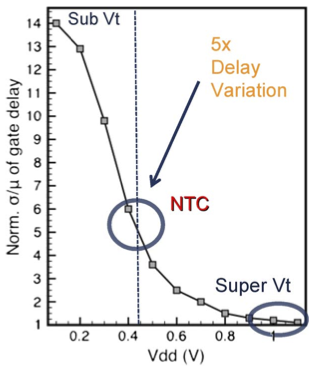
\includegraphics[width=0.4\textwidth]{dreslinski_voltage_delay}
    \caption{Dependence of delay on voltage in near-threshold.~\cite{Dreslinski:2010ez}}
    \label{fig:voltage_delay}
\end{figure}
Because the delay of a gate has a strong dependence on gate voltage in near-threshold operation (see Figure~\ref{fig:voltage_delay}), determining the effect of small changes in $\Delta V_{th}$ is essential to understanding the operation of near-threshold circuits.
This delay is determined by the drain current of the transistor.
The drain current has fundamentally different relationships to voltage in sub- and super-threshold operation; in the sub-threshold mode, the current has an exponential relationship to voltage~\cite{Enz:1995vs} 

\begin{equation}
I_D \propto e^\frac{V_P-V_S}{U_T}
\end{equation}

while super-threshold operation yields a quadratic relationship

\begin{equation}
I_D \propto (V_P-V_S)^2
\end{equation}

where $V_P=V_G-V_{TH}-V_\gamma$ with $V_\gamma$ being a function of body effect.

For near-threshold operation, however, an interpolation has to be used to bridge these two expressions~\cite{Enz:1995vs}, giving us the forward drain current as

\begin{equation}
\label{eqn:nth_current}
I_D \propto \left[\ln\left(1+e^\frac{V_G-V_{TH}-V_\gamma}{2}\right)\right]^2
\end{equation}

The relationship between delay and current, as derived in~\cite{Hanson:2007uu}, is
\begin{equation}
\label{eqn:delay}
t_p = \frac{k_d\cdot C_L\cdot V_D}{I_{on}}
\end{equation}

When Equation~\ref{eqn:nth_current} is combined with Equation~\ref{eqn:delay}, the expression for delay becomes

\begin{equation}
\label{eqn:nth_delay}
t_p\propto\frac{V_D}{\left[\ln\left(1+e^\frac{V_G-V_{TH}-V_\gamma}{2}\right)\right]^2}
\end{equation}
 
 showing that variations in $V_G$ or $V_\gamma$ that are considered insignificant in super-threshold operation can cause large differences in transistor delay.
For example, a 50mV difference in threshold voltage could result in a $7.5\%$ reduction in FMAX and a 50mV difference in $V_G$ can result in a $11\%$ reduction in FMAX; the same difference in $V_G$ at super-threshold results in a $0.7\%$ reduction.

In near-threshold operation even very small differences in voltages and device characteristics, those of a magnitude that can easily be overlooked in super-threshold operation, have a dramatic effect on transistor operating frequency. 
This means that not only does near-threshold operation translate to a slower device, but it also translates to a much more variable device.
Looking at near-threshold as having 10x lower performance is not enough; one must also consider the additional safety factor needed to account for this variation.
